
 
\subsubsection{Geometry and Dynamics }
\index{Mallahi-Karai, Keivan}

\paragraph{Research Team}
Keivan Mallahi-Karai (Visiting Lecturer)

\medskip
 
Arithmetic groups have been a subject of mathematical investigation for over a
century. Various methods, ranging from abstract group theory to ergodic theory
techniques, have been put to use to study this interesting class of groups.
Roughly speaking, the term `arithmetic group' refers to the group of integer
points of an algebraic group ${\bf G}$ which is defined over the field of
rational numbers. A basic and in some sense prototypical example is the group
of integral unimodular matrices ${\rm SL}_n({\bf Z})$.   

My research in the last few years has clustered around studying arithmetic
groups and other groups that look ``arithmetic'' in some way, from various
points of view. One of the  most important properties of arithmetic groups that
was discoverd by David Kazhdan is  known as {\sl property T.} A group $G$ has
property T if, roughly speaking, the trivial representation of $G$ is isolated
in a certain topology defined on the unitary  dual of $G$. Surprisingly, this
property implies really striking algebraic properties  of $G$.

 
\paragraph{Highlights}

My work in this direction is related to the group of tame automorphisms of the
free nilpotent groups. This group consists of those automorphisms of a free
nilpotent group which are induced from the covering free group. If the number
$n$ of the generators of the free group in question exceeds $3$, Lubotzky and
Pak have shown that this group has property~T. One ingenious application of
this result is to obtain the best upper bound for the mixing time of the
product replacement algorithm on finite nilpotent groups which can be may be
used to find a ``random element'' in $G$. This algorithm uses a random walk on
a certain graph $\Gamma (G)$ which is naturally associated to $G$. Mixing time
of this random walk, whose properties are related to representation-theoretic
properties of $G$, is a way of measuring how long we must continue our walk so
that the probability of stopping at any element is close enough to the uniform
distribution.  

Lubotzky and Pak in a ground-breaking work have shown that for a nilpotent group of class $c$ the mixing time is bounded from above by $M(c,k) \log |G|$ where the constant $M(c,k)$ is related to the Kazhdan constant for the group of tame automorphisms of the free nilpotent group. In one of my works, I computed an explicit lower bound for $M(c,k)$ as a function of the number of generators $k$ and the nilpotency class $c$. The main ingredient in this computation is
the following theorem that gives a lower bound for the Kazhdan constants:
 
{\bf Theorem.}
Let $k \ge 4$ be an integer, $F_k$ the free group on $k$ generators, and $S$
the set of Nielsen transformations of $F_k$. Let $A_k(c)$ be the group of tame
automorphisms of the free nilpotent group of class $c$. If $c<2r+1$, then the
Kazhdan constant is bounded from below by $${\mathcal K} (A_k(c), S) \ge 
\frac{1}{4\sqrt{c(84\sqrt{k}+1920)k^c}} $$ 

From here, one can easily derive explicit upper bound for the mixing time of
the product  replacement algorithm on finite nilpotent groups.

The proof of this theorem uses some ideas developed by Y.~Shalom to compute the
Kazhdan  constant for ${\rm SL}_n ({\bf Z})$ along with a theorem of
Furstenberg about invaraint  measures on the projective space and Formanek's
characterization of the center of the automorphism group of the free nilpotent
group.


\begin{figure}[ht]
 \begin{center}
   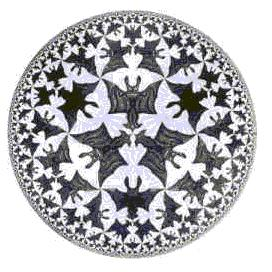
\includegraphics[width=6cm]{Mallahi-Karai/escher.jpg}
   \mycaption{Visual representation of an arithmetic group in Escher's tiling of hyperbolic plane)}\label{fig:escher}
  \end{center}
\end{figure}

